% Q3: Hertzian Dipole — Validity Criterion
% Teaching diagram: compares antenna length to wavelength
\documentclass[border=10pt]{standalone}
\usepackage{tikz}
\usepackage{amsmath, amssymb}
\usetikzlibrary{arrows.meta, decorations.pathreplacing, patterns}

\renewcommand{\familydefault}{\sfdefault}

\begin{document}
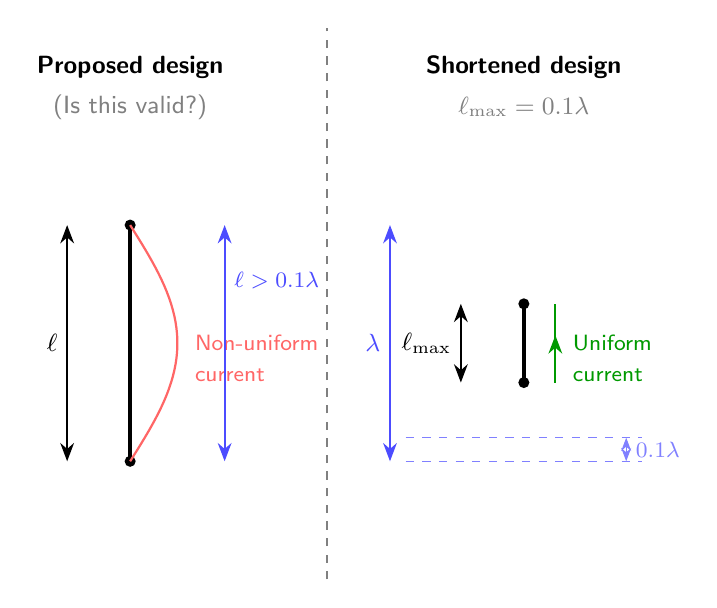
\begin{tikzpicture}[
    every node/.style={font=\sffamily\normalsize},
    >=Stealth
]

% ===== LEFT PANEL: Invalid (current question) =====
\node[font=\sffamily\small\bfseries] at (2, 6.5) {Proposed design};
\node[font=\sffamily\small, gray] at (2, 6.0) {(Is this valid?)};

% --- Antenna (too long) ---
\draw[very thick, black] (2, 1.5) -- (2, 4.5);
\fill[black] (2, 1.5) circle (2pt);
\fill[black] (2, 4.5) circle (2pt);

% --- Current distribution (non-uniform, sinusoidal) ---
\draw[thick, red!60, domain=1.5:4.5, samples=40]
    plot ({2 + 0.6*sin(180*(\x-1.5)/3.0)}, \x);
\node[right, font=\sffamily\footnotesize, red!60] at (2.7, 3.0) {Non-uniform};
\node[right, font=\sffamily\footnotesize, red!60] at (2.7, 2.6) {current};

% --- Length label ---
\draw[<->, thick] (1.2, 1.5) -- (1.2, 4.5);
\node[left, font=\sffamily\small] at (1.2, 3.0) {$\ell$};

% --- Wavelength scale ---
\draw[<->, thick, blue!70] (3.2, 1.5) -- (3.2, 4.5);
\node[right, font=\sffamily\footnotesize, blue!70] at (3.2, 3.8) {$\ell > 0.1\lambda$};


% ===== RIGHT PANEL: Valid (corrected design) =====
\node[font=\sffamily\small\bfseries] at (7, 6.5) {Shortened design};
\node[font=\sffamily\small, gray] at (7, 6.0) {$\ell_{\max} = 0.1\lambda$};

% --- Antenna (short) ---
\draw[very thick, black] (7, 2.5) -- (7, 3.5);
\fill[black] (7, 2.5) circle (2pt);
\fill[black] (7, 3.5) circle (2pt);

% --- Current distribution (approximately uniform) ---
\draw[thick, green!60!black] (7.4, 2.5) -- (7.4, 3.5);
\draw[thick, green!60!black, ->] (7.4, 2.5) -- (7.4, 3.1);
\node[right, font=\sffamily\footnotesize, green!60!black] at (7.5, 3.0) {Uniform};
\node[right, font=\sffamily\footnotesize, green!60!black] at (7.5, 2.6) {current};

% --- Length label ---
\draw[<->, thick] (6.2, 2.5) -- (6.2, 3.5);
\node[left, font=\sffamily\small] at (6.2, 3.0) {$\ell_{\max}$};

% --- Full wavelength scale bar ---
\draw[<->, thick, blue!70] (5.3, 1.5) -- (5.3, 4.5);
\node[left, font=\sffamily\small, blue!70] at (5.3, 3.0) {$\lambda$};

% --- 0.1 lambda marker ---
\draw[thin, dashed, blue!50] (5.5, 1.5) -- (8.5, 1.5);
\draw[thin, dashed, blue!50] (5.5, 1.8) -- (8.5, 1.8);
\draw[<->, thin, blue!50] (8.3, 1.5) -- (8.3, 1.8);
\node[right, font=\sffamily\footnotesize, blue!50] at (8.3, 1.65) {$0.1\lambda$};


% --- Divider ---
\draw[thin, dashed, gray] (4.5, 0) -- (4.5, 7);


\end{tikzpicture}
\end{document}
